\documentclass[a4paper]{article}

\usepackage{algorithm,amsmath}
\usepackage[pdftex]{graphicx}
\usepackage[margin=3.5cm]{geometry}
\usepackage[format=hang,labelfont=it]{caption}
\usepackage[noend]{algorithmic}

\floatname{algorithm}{Listing}
\algsetup{indent=3em}
\renewcommand{\algorithmiccomment}[1]{\quad \{\emph{#1}\}}

\setcounter{page}{3}

\begin{document}

\begin{figure}
  \centering
  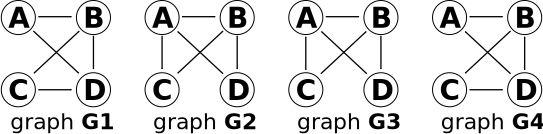
\includegraphics[width=0.55\columnwidth]{q3-graphs.pdf}
  \caption{Example graphs.}\label{fig:a1-graphs}
\end{figure}

\begin{figure}
  \centering
  \fbox{%
    \begin{minipage}[t]{0.3\columnwidth}
      definition \textbf{D1}\\
      \emph{adjacency lists}\\[1.1\baselineskip]
      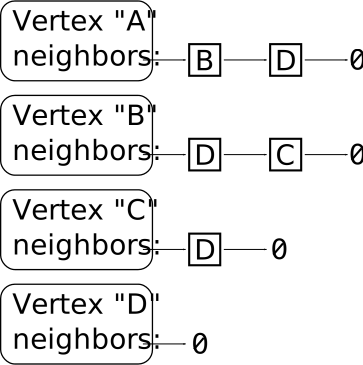
\includegraphics[width=\columnwidth]{q3-adjlist-diagrams.pdf}
    \end{minipage}%
  }
  \fbox{%
    \begin{minipage}[t]{0.3\columnwidth}
      definition \textbf{D2}\\
      \emph{adjacency matrix}\\[1.1\baselineskip]
      \begin{tabular}{|*{5}{c|}}
        \hline
        \emph{source}
        &
        \multicolumn{4}{l|}{\emph{destination}} \\
          & A & B & C & D \\
        \hline
        A &   & * &   &   \\
        \hline
        B &   &   & * &   \\
        \hline
        C &   &   &   & * \\
        \hline
        D & * & * &   &   \\
        \hline
      \end{tabular}
    \end{minipage}}
  \caption{Example representations for two of the graphs from Figure~\ref{fig:a1-graphs}.}\label{fig:a1-reps}
\end{figure}

\begin{figure}
  \centering
  \begin{minipage}{0.4\columnwidth}
    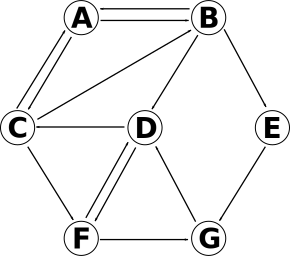
\includegraphics[width=0.75\columnwidth]{q4-graph-diagram.pdf}
  \end{minipage}
  \begin{minipage}{0.45\columnwidth}
    \small
    \begin{tabular}{|*{8}{c|}}
      \hline
      \emph{source}
      &
      \multicolumn{7}{l|}{\emph{destination}} \\
        & A & B & C & D & E & F & G \\
      \hline
      A &   & * & * &   &   &   &   \\
      \hline
      B & * &   &   & * & * &   &   \\
      \hline
      C & * & * &   &   &   & * &   \\
      \hline
      D &   &   & * &   &   & * &   \\
      \hline
      E &   &   &   &   &   &   & * \\
      \hline
      F &   &   &   & * &   &   & * \\
      \hline
      G &   &   &   & * &   &   &   \\
      \hline
    \end{tabular}
  \end{minipage}
  \caption{A graph and its adjacency matrix representation.}\label{fig:a2}
\end{figure}

\begin{figure}
  \centering
  \includegraphics[width=0.35\columnwidth,trim=1cm 1cm 1cm 1cm]{dag-small.pdf}
  \caption{Example DAG arranged from left to right according to topological order.}\label{fig:topo-example}
\end{figure}

\begin{figure}
  \centering
  \begin{minipage}{0.35\columnwidth}
    \centering
    \includegraphics[width=0.7\columnwidth,trim=1cm 1cm 1cm 1cm]{cycle-detection-dag.pdf}\\
    \textbf{graph A}
  \end{minipage}
  \begin{minipage}{0.35\columnwidth}
    \centering
    \includegraphics[width=0.7\columnwidth,trim=1cm 1cm 1cm 1cm]{cycle-detection-non-dag.pdf}\\
    \textbf{graph B}
  \end{minipage}
  \caption{Example graphs for topological ordering.}\label{fig:a3-graphs}
\end{figure}

\small

\begin{algorithm}
  \caption{
    Breadth-first search: \textbf{BFS}($G,n$)\\
    \textbf{Input:} a directed graph $G$ and a start vertex $n$
  }\label{algo:bfs}
  \begin{algorithmic}
    \STATE $Q \leftarrow$ empty queue \COMMENT { vertices to be processed }
    \STATE $V \leftarrow$ empty set \COMMENT { visited vertices }
    \STATE enqueue $n$ onto $Q$
    \STATE add $n$ to $V$
    \WHILE { $Q \neq \emptyset$ }
      \STATE $t \leftarrow \text{dequeue}(Q)$
      \STATE process $t$ \COMMENT { e.g.\ print its data }
      \FORALL[visit all outgoing edges] { edges $(t,u)$ }
        \IF[found an unvisited vertex] { $u \notin V$ }
          \STATE add $u$ to $V$
          \STATE enqueue $u$ onto $Q$
        \ENDIF
      \ENDFOR
    \ENDWHILE
  \end{algorithmic}
\end{algorithm}

\begin{algorithm}
  \caption{
    Depth-first search: \textbf{DFS}($G,n$)\\
    \textbf{Input:} a directed graph $G$ and a start vertex $n$\\
    \textbf{Initializations} before calling DFS(): an initially empty set of discovered vertices $D$ and an initially empty set of explored edges $E$
  }\label{algo:dfs}
  \begin{algorithmic}
    \STATE process $n$ \COMMENT { e.g.\ print its data }
    \STATE add $n$ to $D$ \COMMENT { label it ``discovered'' }
    \FORALL[visit all outgoing edges] { edges $e=(n,m)$ }
      \IF[found an unexplored edge] { $e \notin E$ }
        \STATE add $e$ to $E$ \COMMENT { label it ``explored'' }
        \IF[found an undiscovered vertex] { $m \notin D$ }
          \STATE recursively call \textbf{DFS}($G,m$)
        \ENDIF
      \ENDIF
    \ENDFOR
  \end{algorithmic}
\end{algorithm}

\begin{algorithm}
  \caption{
    Kahn's Algorithm\\
    \textbf{Input:} a directed graph $G$
  }\label{algo:kahn}
  \begin{algorithmic}
    \STATE $L \leftarrow$ empty list \COMMENT { will contain the topological order }
    \STATE $S \leftarrow$ set of nodes that have \textbf{no incoming} edges
    \WHILE { $S \neq \emptyset$ }
      \STATE remove a node $n$ from $S$
      \STATE insert $n$ into $L$
      \FORALL [visit all outgoing edges] { edges $e = (n,m)$ }
        \STATE remove $e$ from $G$
        \IF { $m$ has no more incoming edges }
          \STATE insert $m$ into $S$
        \ENDIF
      \ENDFOR
    \ENDWHILE
    \IF { $G$ has edges }
      \RETURN error \COMMENT { $G$ has at least one cycle }
    \ENDIF
    \RETURN $L$
  \end{algorithmic}
\end{algorithm}



\end{document}
